\documentclass[a4paper, notitlepage]{report}

%====================== PACKAGES ======================

\usepackage[english]{babel}
\usepackage[utf8]{inputenc}

\usepackage[sorting=none]{biblatex}
\usepackage{csquotes}
\bibliography{bibliographie}


%pour gérer les positionnement d'images
\usepackage{float}
\usepackage{amsmath}
\usepackage{graphicx}
\usepackage{braket}
\usepackage[colorinlistoftodos]{todonotes}

\usepackage{xcolor}
\definecolor{ups}{RGB}{86,08,59}
\definecolor{cs}{RGB}{148,13,56}

\usepackage{url}
%pour les informations sur un document compilé en PDF et les liens externes / internes
\usepackage{hyperref}
\hypersetup{%
  colorlinks=false,% hyperlinks will be black
  linkbordercolor=cs,% hyperlink borders will be red
  urlbordercolor=cs,% hyperlink borders will be red
  citebordercolor=cs,
%   pdfborderstyle={/S/U/W 1}% border style will be underline of width 1pt
}
%pour la mise en page des tableaux
\usepackage{array}
\usepackage{tabularx}
%espacement entre les lignes
\usepackage{setspace}
\usepackage{svg}

\usepackage{wrapfig}
\usepackage{multicol}

% Special symbols
\usepackage{amssymb}
\usepackage{mathrsfs}

%police et mise en page (marges) du document
\usepackage[T1]{fontenc}
\usepackage[top=2cm, bottom=2cm, left=2cm, right=2cm]{geometry}
%Pour les galerie d'images
\usepackage{subfig}
\usepackage{tikz}
\usetikzlibrary{positioning}
\usetikzlibrary{calc}
\usepackage{tikz-cd}

% Algorithms
\usepackage{algorithm}
\usepackage{algpseudocode}
\usepackage{listings}
\renewcommand\lstlistingname{Programme}
\renewcommand\lstlistlistingname{Liste des programmes}
\definecolor{codegreen}{rgb}{0,0.6,0}
\definecolor{codegray}{rgb}{0.5,0.5,0.5}
\definecolor{codepurple}{rgb}{0.58,0,0.82}
\definecolor{backcolour}{rgb}{0.95,0.95,0.92}
\lstdefinestyle{mystyle}{
    commentstyle=\color{ups},
    keywordstyle=\color{cs},
    numberstyle=\tiny\color{codegray},
    stringstyle=\color{ups},
    basicstyle=\ttfamily,
    breakatwhitespace=false,
    breaklines=true,
    captionpos=b,
    keepspaces=true,
    numbersep=5pt,
    showspaces=false,
    showstringspaces=false,
    showtabs=false,
    tabsize=2
}

\lstset{style=mystyle}


% No new page after chapter
\usepackage{etoolbox}
\makeatletter
\patchcmd{\chapter}{\if@openright\cleardoublepage\else\clearpage\fi}{}{}{}
\makeatother

\newcommand{\RE}{\mathrm{Re}}
\newcommand{\IM}{\mathrm{Im}}
\newcommand{\function}[5]{\begin{array}{l|rcl}
#1: & #2 & \longrightarrow & #3 \\
    & #4 & \longmapsto & #5 \end{array}}
\newcommand{\mathsc}[1]{{\normalfont\textsc{#1}}}
\newcommand*{\toccontents}{\@starttoc{toc}}

%====================== INFORMATION ET REGLES ======================

%rajouter les numérotation pour les \paragraphe et \subparagraphe
\setcounter{secnumdepth}{4}
\setcounter{tocdepth}{4}



%======================== DEBUT DU DOCUMENT ========================

\begin{document}

%régler l'espacement entre les lignes
\newcommand{\HRule}{\rule{\linewidth}{0.5mm}}

%page de garde
\begin{center}

% Upper part of the page. The '~' is needed because only works if a paragraph has started.
\includesvg[width=\textwidth]{./figures/Logo}~\\[1cm]

% \textsc{\LARGE CentraleSupélec}\\[1.5cm]

\textsc{\Large }\\[0.5cm]

% Title
\HRule \\[0.4cm]

{\huge \bfseries Around Quantum Decision Diagrams\\
[0.4cm] }

{\large \bfseries Report -- Research Track -- Semester 7\\[0.4cm] }
{\large \bfseries \textsl{Student : Malo \textsc{Leroy}}\\ }
{\large \bfseries \textsl{Supervisor : Renaud \textsc{Vilmart}}\\[0.4cm] }


\HRule \\[1.5cm]

\begingroup
\let\clearpage\relax
\tableofcontents
\endgroup

\vfill

% Bottom of the page
{\large {February 17${}^\text{th}$ 2025}}

\end{center}

%page blanche
%\newpage
%~
%ne pas numéroter cette page
\thispagestyle{empty}


\thispagestyle{empty}
\setcounter{page}{0}
%ne pas numéroter le sommaire

%\newpage

%espacement entre les lignes d'un tableau
\renewcommand{\arraystretch}{1.5}

%====================== INCLUSION DES PARTIES ======================

~
\thispagestyle{empty}
%recommencer la numérotation des pages à "1"
\setcounter{page}{0}
\newpage

\chapter{Introduction} % 1 page max
\label{ch:Introduction}


\section{Context and objective}
\label{sec:Contexte}

\textbf{Quantum computing} is a rapidly expanding field. This technology, which enables qubits to be manipulated instead of the bits that form the basis of today's computing, paves the way for algorithms that are more powerful than conventional ones. As the quantum machines running these algorithms are still under development and costly, there is a need for tools to simulate and verify quantum algorithms using classical machines. The aim of this project is to propose a model of the data structure of abstract additive quantum decision diagrams, based on existing work, and to simulate them in order to study their performance.


\section{State of the art}
\label{sec:Etat}


\subsubsection*{Quantum computing}

The first postulate of quantum physics, the \textbf{principle of superposition}, states that the state space of a quantum system is a Hilbert space. Consequently, while a \textit{bit} can classically only be in a $\ket 0$ or $\ket 1$ state, its quantum counterpart, the \textbf{qubit}, can be in a superposition of these two states.
$$\ket \psi = \alpha \ket 0 + \beta \ket 1$$

\noindent where $\alpha, \beta$ are complex coefficients. The second postulate, the \textit{measurement principle}, states that when a qubit is measured, it is projected onto one of the base states $\ket 0$ or $\ket 1$ with probability $|\alpha|^2$ or $|\beta|^2$ respectively.

States with $n$ qubits can be represented by $2^n$-dimensional \textbf{vectors}, the states of the set consisting of two systems being those obtained by tensor product (\textit{Kronecker product}) of a state of the first system and a state of the second. It is this exponential number of complex parameters for a multi-qubit state that makes the classical study of quantum algorithms difficult, since the states take up exponentially large amounts of memory.

\vspace{1em}

As in classical computing, elementary operations on memory are performed in quantum computing by \textbf{gates}. From a mathematical point of view, a gate operating on $n$ qubits is commonly represented by a matrix of size $2^n \times 2^n$. Applying a gate $M$ to a set of qubits $v$ then amounts to multiplying the state vector by the gate matrix.

Parallel application of multiple gates to multiple qubits is represented by the \textbf{tensor product} (Kronecker product) of the gate matrices. It should be noted, however, that the application of gates to qubits in this way takes exponential time as a function of the number of qubits, making the naive use of quantum algorithms on classical machines inefficient.

The application of gates to qubits is frequently represented as \textbf{quantum circuits}, where qubits are represented by lines and gates by boxes.

\begin{figure}
  \centering
  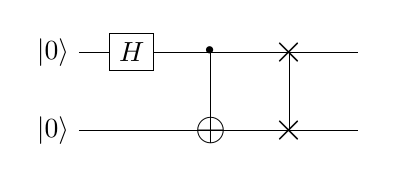
\begin{tikzpicture}
    \node (end1) at (4, 0) {};
    \node (end2) at (4, -1) {};
    \node (q1) at (0, 0) {$\ket 0$};
    \node (q2) at (0, -1) {$\ket 0$};

    \node [draw] (h1) at (1, 0) {$H$};
    \draw (q1) -- (h1);
    \draw (h1) -- (end1);
    \draw (q2) -- (end2);
    \node (cx) at (2, -1) {\Large $\oplus$};
    \node (cx2) at (2, 0) {\Huge $\cdot$};
    \node (s1) at (3, 0) {\Large $\times$};
    \node (s2) at (3, -1) {\Large $\times$};

    \draw (s1.center) -- (s2.center);
    \draw (cx2.center) -- (cx.center);
  \end{tikzpicture}
  \caption{2-qubits circuit with gates $H$, $CX$ and $S$}
\end{figure}

Any \textit{unitary} and \textit{reversible} matrix can be used as a quantum gate. Among the most common gates are the Hadamard gate ($H$), the “not” gate ($X$), the “controlled not” gate ($CX$), or the swap gate ($S$). These and other gates are used in quantum algorithms such as Deutsch-Josza's \cite{DJ_1992}, Grover's \cite{Grover_1996} and Shor's \cite{Shor_1997}.

\vspace{1em}

To provide a unified language for developing quantum algorithms from gates that can be interpreted on any hardware, IBM released the \textbf{Open QASM} programming language in 2017. \cite{QASM_2017} It defines qubits on which gates are applied, and the program can then be simulated or executed on a quantum computer as on a conventional computer. The preceding circuit can, for example, be represented by the program \ref{lst:QASM}:

\begin{figure}[thp]
  \renewcommand{\figurename}{Program}
  \centering
\begin{tabular}{c}
\begin{lstlisting}
  qubit a;
  qubit b;
  h a;
  cx a b;
  s a b;
\end{lstlisting}
\end{tabular}
\caption{Example Open QASM code}
\label{lst:QASM}
\end{figure}

\subsubsection*{Decision diagrams}

The \textbf{decision diagram} structure is a data structure developed in the 1970s. It has since become widely used in computer science, in particular to make the representation of binary functions more compact.

Take, for example, the binary function $f(x_1, x_2, x_3) = x_1 \lor (x_2 \land x_3)$. In the general case, such a function is represented using a \textit{truth table}, i.e. in a size that grows exponentially with the number of binary variables considered. A more compact representation can be achieved using a decision diagram, as shown in \autoref{fig:ExempleDD}, where left-hand children are indicated by dotted arrows and right-hand children by solid arrows.

\begin{figure}
  \renewcommand{\arraystretch}{0.8}% Tighter
  \begin{tabular}{c|c|c|c}
    $x_1$ & $x_2$ & $x_3$ & $f(x_1, x_2)$ \\
    \hline
    0 & 0 & 0 & 0 \\
    0 & 0 & 1 & 0 \\
    0 & 1 & 0 & 0 \\
    0 & 1 & 1 & 1 \\
    1 & 0 & 0 & 1 \\
    1 & 0 & 1 & 1 \\
    1 & 1 & 0 & 1 \\
    1 & 1 & 1 & 1
  \end{tabular}
  \hfill{}
  % https://tikzcd.yichuanshen.de/#N4Igdg9gJgpgziAXAbVABwnAlgFyxMJZAJgBoAGAXVJADcBDAGwFcYkQAPAfQEYACADoDGEAE58AFN2KDh9MFD7cAzAEoQAX1LpMufIRTLSy6nSat2PTdpAZseAkXIVTDFm0QgpvdVp339J1IeV3MPL2lfGzs9RxRnYlD3dm81a39Yg2QeYySLT3J0210HLJyQmjd8zi4ZIUZ5RRUimNKiMkTKsPZmjVMYKABzeCJQADNRCABbJGcQHAgkADYaRiwwcKh6OAALAaKJ6dmaBaQckAAjGAUkZTmq8O5+AF4+Kz8QQ5nEFfnFxAArKt1pttnsoCAuslPNJnoVVvQrowAAolQKeURYQY7HAHSbfX6nRAAdih1Vh7xsXyQpL+SCBIDWG3YW12+zJjy4yj4r0KH2pJJO-3ODx6XOe70oGiAA
  \begin{tikzcd}[column sep=tiny]
    (x_1) &                                                                & x_1 \lor (x_2 \land x_3) \arrow[ld, dashed] \arrow[rddd, "x_1 = 1", bend left] &   \\
    (x_2) & x_2 \land x_3 \arrow[dd, "x_2=0"', dashed] \arrow[rd, "x_2=1"] &                                                                                &   \\
    (x_3) &                                                                & x_3 \arrow[ld, "x_3 = 0", dashed] \arrow[rd, "x_3=1"]                          &   \\
          & 0                                                              &                                                                                & 1
    \end{tikzcd}
    \hfill{}
  % https://tikzcd.yichuanshen.de/#N4Igdg9gJgpgziAXAbVABwnAlgFyxMJZARgBoAGAXVJADcBDAGwFcYkQQBfU9TXfQigBMpAMzU6TVu2JceIDNjwEi5MRIYs2iEOTm8lA1aWIap2jtwP8VKMkLNb2XCTCgBzeEVAAzAE4QALZIaiA4EEiiNIxYYBZQ9HAAFm76IP5BITThSGQgAEYwYFCR5FbpAcGIUWERiCIgMXHsCcmp0fSFjAAKfMqCIH5Y7kk4aRlVNTmIACzlE0gz2XUNTfGJKSXzlYvLuZyUnEA
  \begin{tikzcd}[column sep=huge, row sep=large]
    & {} \arrow[ld, dashed] \arrow[rddd, bend left] &   \\
  {} \arrow[dd, dashed] \arrow[rd] &                                               &   \\
    & {} \arrow[ld, dashed] \arrow[rd]              &   \\
  0                                &                                               & 1
  \end{tikzcd}

  \caption{(a) Table de vérité (b) Diagramme de décision (c) Diagramme de décision sans labels}
  \label{fig:ExempleDD}
\end{figure}

Decision diagrams take advantage of the data's internal \textbf{structure} (here, a Boolean function). On the one hand, labels are not needed to reconstruct the values taken by the function.
On the other hand, in the worst case, i.e. where the function has no structure allowing reduction, the size of the decision diagram (its number of branches) is $2^{n+1} - 2$ which, like the number of values $2^n$ to be stored in a truth table, is \textbf{exponential} in $n$. In the worst case, decision diagrams offer no improvement, but are not asymptotically worse than truth tables either.

\subsubsection*{Abstract interpretation}

Abstract interpretation is a general method of dealing with the properties of computer programs by abstracting them. It was introduced by Patrick and Radhia Cousot in 1977 \cite{CousotCousot77-1}. It can also be used to solve problems or compute faster.

Consider the following problem: we're trying to determine the sign of the expression $-12 \times 7 - 13$. We could calculate the result of this expression, but we could also note that $-12$ and $-13$ are negative and that 7 is positive, hence $-12 \times 7$ is negative, so the expression is negative. More formally, we've taken the concrete elements $-12$, 7 and $-13$ and replaced them with the abstract elements $\oplus$ “positive” and $\ominus$ “negative”, on which we define sum and product operations according to well-known rules.

There are many uses for the abstract interpretation \cite{Rosendahl_1995}, for example in program compilation. In this project, we'll be using it to reduce quantum decision diagrams, even if this means losing some of the information they contain. This is also the case for the previous example: abstracting elements by their sign does not always allow us to determine the sign of the expression.


\section{Contribution}
\label{sec:Contribution}

The various concepts presented in the state of the art can all be used to improve the computation speed or memory size of a dataset. The aim of this project was therefore to combine these concepts, adding an extra dimension, additivity: the fact that a diagram has several right (respectively left) wires, the interpretation being that the “effective right wire” is the sum of the diagram's right (respectively left) wires.
The aim of the project was therefore to propose a model of abstract, additive quantum decision diagrams, and to simulate them in order to study their performance in comparison with other models.

As a preliminary step, a study of polar complex intervals was carried out, which had not been done in the literature until now.
A mathematical \textbf{model} of the data structure and reduction methods were formalized, and reduction algorithms were developed to reduce these diagrams.
In addition, methods for applying quantum gates to the diagrams have been formalized.
An \textbf{implementation} of these algorithms was carried out, without relying on existing libraries (except for unit tests).

\section{Structure of the report}
\label{sec:Structure}

\autoref{ch:Modele} presents the theoretical model of quantum decision diagrams that has been developed, including the accompanying reduction and gating algorithms. Next, \autoref{ch:Implementation} discusses the implementation carried out. Finally, a short conclusion is presented in \autoref{ch:Conclusion}.

A more complete theoretical document is available online. Some theoretical points succinctly presented in this report, or theorems whose proof is not specified, are detailed in this document. \cite{Leroy_2025} In addition, technical documentation of the code is available online. \cite{Leroy_doc}


\newpage

\newpage

\chapter{Modèle théorique}
\label{ch:Modele}

Le modèle théorique proposé est celui des \textbf{diagrammes de décision quantiques additifs abstraits}.

\section{Arithmétique des intervalles}
\label{sec:ArithmetiqueIntervalles}

L'arithmétique des intervalles dans le cadre de l'interprétation abstraite est proche de l'exemple de calcul sur les signes de la \autoref{sec:Etat}. L'arithmétique des intervalles est utilisée pour déterminer un ensemble de valeurs possibles pour une expression mathématique en utilisant des intervalles pour les valeurs des variables.

L'arithmétique des intervalles réels a été étudiée \cite{Sunaga_2009}, et l'arithmétique des intervalles complexes cartésien a fait l'objet d'études légères par le passé \cite{Rokne_1971}. Au cours de ce projet, un travail a été réalisé pour explorer les possibilités de l'arithmétique des \textbf{intervalles complexes cartésiens et polaires}.

\begin{figure}
  \centering
  \resizebox{.5\textwidth}{!}{
  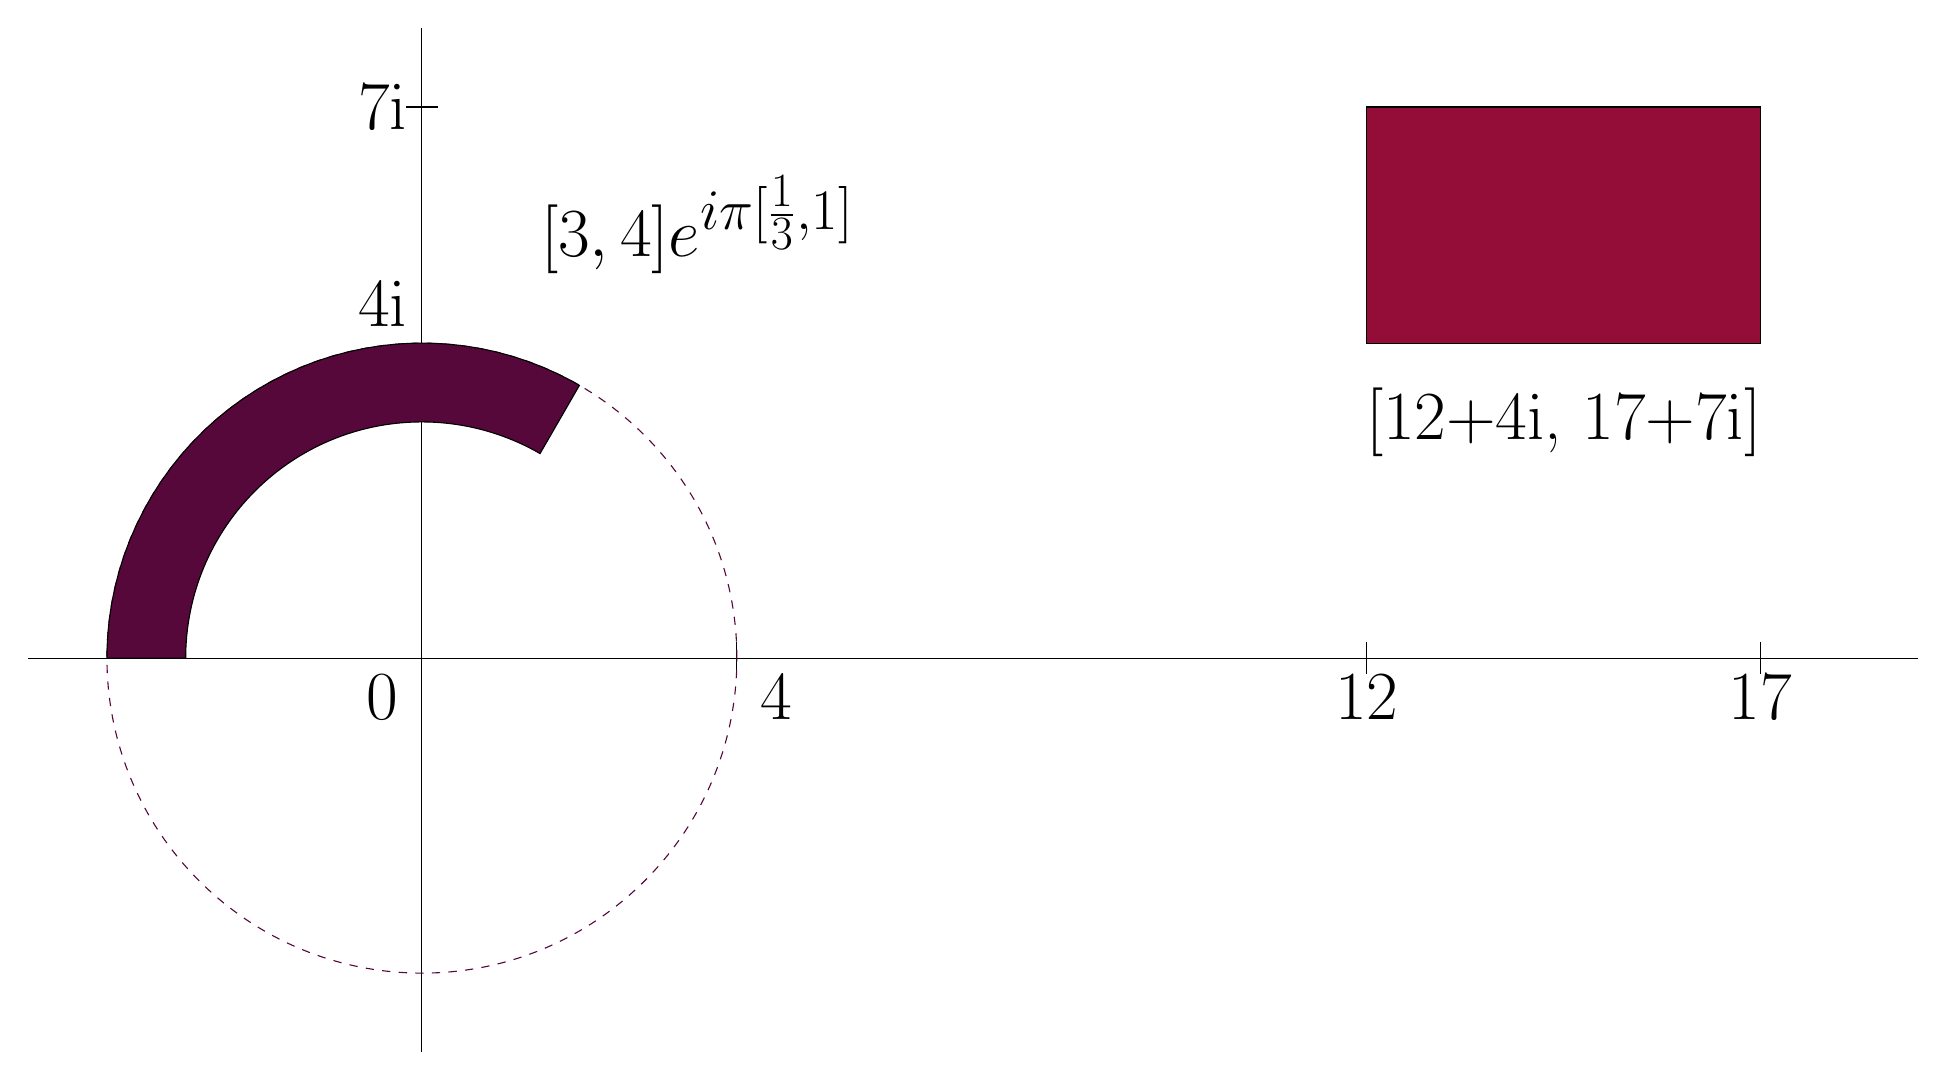
\begin{tikzpicture}
    \coordinate (c) at (0,0);
    \tikzstyle{every node}=[font=\Huge]
    \draw [fill=cs] (12,4) rectangle (17,7);
    \node at (14.5,3) {[12+4i, 17+7i]};
    \draw (-5,0) -- (19,0);
    \draw (0,-5) -- (0,8);

    \draw (4,-.2) -- (4,.2);
    \node at (4.5,-.5) {4};

    \draw (-.2,4) -- (.2,4);
    \node at (-.5, 4.5) {4i};

    \draw (-.2, 7) -- (.2, 7);
    \node at (-.5,7) {7i};

    \draw (12,-.2) -- (12,.2);
    \node at (12,-.5) {12};

    \draw (17,-.2) -- (17,.2);
    \node at (17,-.5) {17};

    \node at (-.5,-.5) {0};

    \draw [color=ups,dashed] (c) circle (4cm);
    \node at (3.5,5.5) {$[3, 4]e^{i\pi[\frac 1 3, 1]}$};
    \draw[fill=ups]
    ($(c) + (60:4cm)$) arc (60:180:4cm)
    --
    ($(c) + (180:3cm)$) arc (180:60:3cm)
    -- cycle;
  \end{tikzpicture}
  }
  \caption{Exemple d'intervalles complexes cartésiens et polaires}
  \label{fig:intervalles}
\end{figure}

Les intervalles complexes cartésiens sont définis par un intervalle pour la partie réelle et un intervalle pour la partie imaginaire. De manière équivalente, ils sont définis comme le plus petit rectangle dans le plan complexe (orienté selon les axes réel et imaginaire) contenant deux complexes. Les intervalles complexes polaires sont définis par un intervalle pour le module et un intervalle pour l'argument. Ces deux types d'intervalles ont des représentations différentes dans le plan complexe, comme le montre la \autoref{fig:intervalles}. Dans un cas comme dans l'autre, l'équivalent abstrait d'une \textbf{opération} $*$ est défini sur des éléments $\alpha$ et $\beta$ de l'ensemble des intervalles cartésiens $\mathcal{A}_0$ ou polaires $\mathcal S_0$ par
$$\alpha * \beta = \bigcap_{\gamma \supset \alpha \circledast \beta\text{ et }\gamma \in \mathcal{A}_0} \gamma \quad \text{où} \quad \alpha \circledast \beta = \{a * b ; a \in \alpha, b \in \beta\}$$

Les opérations de somme, de produit et d'union ainsi construites sont \textbf{sur-approximées} : elles garantissent que l'ensemble des valeurs possibles est inclus dans l'ensemble abstrait, et d'avoir un intervalle pour résultat. Ces opérations ont des propriétés, de distributivité par exemple, parfois très différentes des nombres complexes qu'ils représentent. Des propriétés sur les intervalles cartésiens et polaires sont énoncées et démontrées dans le document annexe \cite{Leroy_2025}.

D'un point de vue pratique, les intervalles cartésiens sont généralement plus simples à manipuler que les intervalles polaires, et sont largement plus adaptés à une structure additive. Les intervalles polaires ont des avantages pour les opérations de multiplication et de division, mais rendent la somme coûteuse en calculs et en perte de précision.

\section{États abstraits et diagrammes}

Les \textbf{états} abstraits à $n$ qubits sont définis comme des $2^n$-uplets d'intervalles complexes, on note leur ensemble $\mathcal A_n$.
Il peut s'agit des intervalles cartésiens ou polaires, puisque les opérations sont définies de manière similaire, mais en pratique on se limite souvent aux intervalles cartésiens.
On définit sur les états la relation d'ordre d'inclusion des états par l'inclusion des produits cartésiens des intervalles les composant.

Les \textbf{diagrammes} sont définis de manière récursive. Le seul diagramme de hauteur 0 est $\boxed 1$, puis si l'ensemble $\mathcal D_n$ des diagrammes de hauteur $n$ est défini, les diagrammes de hauteur $n+1$ peuvent avoir un nombre fini de fils gauches dans $\mathcal D_n$ et un nombre fini de fils droits dans $\mathcal D_n$, chacun étant associé à une amplitude abstraite sur la branche dans $\mathcal A_0$
$$\mathcal{D}_{n+1} = \mathscr{P}_f(\mathcal{A}_0 \times \mathcal{D}_n) \times \mathscr{P}_f(\mathcal{A}_0 \times \mathcal{D}_n)$$

On peut ainsi définir la fonction d'évaluation $\mathcal E : \mathcal D_n \to \mathcal A_n$ sur les diagrammes (une définition similaire est possible en utilisant les intervalles polaires), ce qui permet de définir une relation d'ordre $\le$ sur les diagrammes par inclusion des ensembles abstraits qu'ils représentent.

\section{Approximations}

L'un des objectifs pour cette structure de données est de transformer un diagramme en un autre incluant le diagramme initial et de taille plus faible. Sur les diagrammes de décision abstraits ont été développés deux algorithmes, à partir d'une relation de fusion.

Puisque traiter les diagrammes de manière globale est difficile, on réalise les approximations de manière locale. Plus formellement, une \textbf{approximation globale} est une fonction $g : \mathcal D_n \to \mathcal D_n$ telle que
$$\forall D \in \mathcal D_n, D \le g(D)$$

En pratique, on a surtout développé une \textbf{approximation par fusion}, qui est une fonction $f : \mathcal D_n \times \mathcal D_n \rightarrow \mathcal D_n$ telle que
$$\begin{cases}
  \forall A \not= B \in \mathcal{D}_n, A \le f(A, B)~\text{and}~B \le f(A, B) \\
  \forall A \in \mathcal{D}_n, f(A, A) = A
\end{cases}
$$

Le \textbf{théorème de fusion} indique que si l'on dispose d'une approximation par fusion, alors on dispose d'une approximation globale. Il simplifie grandement les preuves ultérieures, puisque l'on peut se contenter de démontrer la propriété d'approximation par fusion pour montrer l'approximation globale.

D'un point de vue computationnel, les approximations par fusion ont aussi l'avantage de pouvoir s'appliquer à des sous-diagrammes : pour réduire un diagramme $D$, il suffira alors de réaliser une approximation par fusion sur deux sous-diagrammes de $D$. Il est alors possible de réduire un diagramme de manière locale, ce qui est plus efficace que de considérer le diagramme parent directement.

\section{Réduction}

Deux algorithmes de réduction ont été développés, utilisant largement l'approximation par fusion fm (pour \textbf{force merge}) de la \autoref{fig:fm}, qui est centrale dans la réduction des diagrammes.

\begin{figure}[H]
  \centering
% https://tikzcd.yichuanshen.de/#N4Igdg9gJgpgziAXAbVABwnAlgFyxMJZAJgBoAGAXVJADcBDAGwFcYkQBBEAX1PU1z5CKACwVqdJq3YAhHnxAZseAkXKliEhizaIQjAPrl5-ZUKJlNNbdL2HgYALQBGbicUCVw5GKuSd7ABORu5KgqooAGwaWlK6IMHAALYubrym4d4A7DHWceyGxukeZhHIAJy5-rb6Bg6poZ7mKM7OVTbxwUUKYV5EzgDM7fl6iSmujaXezupUeQF6AMIABAC8ywA6GzgwAB44wABmSdwAFBykyzIAlJOZRNHOsQsgd30oABykT-M1PBIwKAAc3gRFAh0CECSSHUIBwECQZH0WDA8Sg9DgAAtAe4IVCYTR4UghsjUex0ViccU8dDEEiiYgSYwUWiIDgdlAQDRsfROXpIGTqZDaW04Qi6TRmWS9BTsZyhfjEKKGUyWeSMXLccKCWKkCIFSLCeL9QoaTqGQBWA16o1IC3cmC89gCtiStUytkcrWK5Xiq2m7WIaK6xA5Ums9k4h1O-kENjWxBfEOVEA8vngONc8Pkz1UgM+2EMsNStEavPgwMzW2JhNV5O131IZxIks55gAI0YrtTjr5YGYjEYhPoWEYzszv3iWx2+2Ap2O1zS+ZFhfFwdbMrL8so3CAA
\begin{tikzcd}[column sep=0.6cm]
  &  & A \arrow[lldd, dashed] \arrow[dd, dashed] \arrow[rrdd] \arrow[rrrrdd] &  & B \arrow[lllldd, dashed] \arrow[lldd, dashed] \arrow[dd] \arrow[rrdd] &  &                                          &                                 &    &         & {\text{fm}(A, B)} \arrow[ldd, dashed] \arrow[rdd] \arrow[rrrdd] \arrow[llldd, dashed] &                                 &  &         \\
  &  &                                                                       &  &                                                                       &  & {} \arrow[rr, "\text{(fm)}", Rightarrow] &                                 & {} &         &                                                                                           &                                 &  &         \\
l_0 \arrow[rr, no head, dotted] &  & l_{n-1}                                                               &  & r_0 \arrow[rr, no head, dotted]                                       &  & r_{m-1}                                  & l_0 \arrow[rr, no head, dotted] &    & l_{n-1} &                                                                                           & r_0 \arrow[rr, no head, dotted] &  & r_{m-1}
\end{tikzcd}
\caption{Approximation par fusion forcée}
\label{fig:fm}
\end{figure}

\noindent où si ampl(A, $x$) est l'amplitude abstraite sur le lien entre $A$ et $x$, alors les nouvelles amplitudes abstraites sont définies par la formule suivante
$$\forall x \in \{l_0, ..., l_{k-1}, r_0, ..., r_{m-1}\},~\text{ampl}(\text{fm}(A, B), x) = \text{ampl}(A, x) \sqcup \text{ampl}(B, x)$$

\noindent où $\sqcup$ est l'opération d'union des intervalles complexes (cartésiens ou polaires). Cette approximation par fusion fonctionne en pratique y compris sur des diagrammes n'ayant a priori pas de descendance commune, puisqu'il suffit d'ajouter des branches avec un poids nul pour se ramener à ce cas. On remarque que cette généralisation ne fonctionne que dans le cas où on permet l'utilisation de diagrammes additifs.

\begin{multicols}{2}
  \section{Exemple d'approximation}
  Considérons le diagramme suivant, où tous les fils (gauche ou droit) sont $\boxed 1$ et où les branches sans amplitude écrite sont d'amplitude 1. Appliquer fm sur $A$ et $B$ permet fait passer le diagramme additif initial à un diagramme additif abstrait $D' \ge D$.

  Ici, la fusion permettrait ensuite de fusionner les deux branches gauches de $D'$ pour obtenir un diagramme non additif, comme le montre la \autoref{fig:exemple_fusion}.

  \columnbreak
  \begin{figure}[H]
    \centering
  % https://tikzcd.yichuanshen.de/#N4Igdg9gJgpgziAXAbVABwnAlgFyxMJZARgBoAGAXVJADcBDAGwFcYkQAREAX1PU1z5CKAEyli1Ok1bsAQjz4gM2PASLlxkhizaIQAQQX8VQomRFbpukAB0bAIwgAPGFAAExHpNcBzeEVAAMwAnCABbJA0QHAgkMikddiwjEBDwyJoYpDEQRiwwayh6OAALVxAabRk9ABZkmkZ6exhGAAUBVWEQYKwfEpwUtIjEKKzEeOawKCQAWhqATgb8wuKy6d4g0OGcsYBmGknpxDnF3OX2ItLyhqaW9pM1PR6+gcqrdjsQ+gBjAFYRQZbOKZWKIfZnAoXVbXBLVEAAm7NNodUxPXr9QHpcYgpDgw5IBYbVJAxA7UG7biUbhAA
  \begin{tikzcd}
    & D \arrow[rd, "i"] \arrow[ld, "4i"', dashed] \arrow[rd, dashed, bend right=49] &                                                     \\
  A \arrow[rd, "\frac52"', dashed, bend right=49] \arrow[rd] &                                                                               & B \arrow[ld, "2"', dashed] \arrow[ld, bend left=49] \\
    & \boxed 1                                                                      &
  \end{tikzcd}
  $\Rightarrow$
  % https://tikzcd.yichuanshen.de/#N4Igdg9gJgpgziAXAbVABwnAlgFyxMJZABgBpiBdUkANwEMAbAVxiRABEQBfU9TXfIRRkATFVqMWbADrSARhAAeMKAAIAjN14gM2PASJl14+s1aIQAYW7iVAc3hFQAMwBOEALZIR1HBCTq1HIwYFBIACwAnNSmUhaaPC7uXog+IH4B1AxYYOYgUHRwABYqIEEhYYgAtFExknnIPqqybnQAxgCsYmUgDHTBDAAK-PpCIK5YdkU4WkmeSGTp-qnloUg10b05eQXFpXVmbOFYPX0Dw3qCbBNTM4kgbvOIixkrW7lsuyVhq5UAzMR7o8Ui9lmlgmtELUJIcLCcuBQuEA
  \begin{tikzcd}[row sep=large]
    D' \arrow[d, "4i"', dashed, bend right=49] \arrow[d, dashed, bend left] \arrow[d, "i", bend left=49] \\
    C \arrow[d, "1", bend left=49] \arrow[d, "{[2, \frac52]}"', dashed, bend right=49]                  \\
    \boxed 1
  \end{tikzcd}
  \caption{Fusion de $A$ et $B$}
  \label{fig:exemple_fusion}
  \end{figure}

  \end{multicols}

\section{Erreur}

S'il est possible de réaliser des fusions sur n'importe quelle paire de diagrammes de même hauteur, savoir lesquels fusionner afin de réduire le diagramme sans causer de trop grande perte de précision est un enjeu majeur. On a donc développé une grandeur d'\textbf{erreur}, qui permet de déterminer si une fusion est intéressante ou non. Cette grandeur se distingue en deux intervalles : $\rho$ et $\varepsilon$, définis inductivement sur les diagrammes de hauteur $n$ par
$$\rho(\boxed{1}) = \{1\}$$
$$\varepsilon(\boxed{1}) = \{0\})$$

$$\forall G, D \in \mathscr{P}_f(\mathcal{A}_0 \times \mathcal{D}_n),
\rho((G, D))
= \left(\sum_{(l, L) \in G} l \rho(L) \right) \bigsqcup \left(\sum_{(r, R) \in D} r \rho(R) \right)$$

\begin{multline*}
\forall G, D \in \mathscr{P}_f(\mathcal{A}_0 \times \mathcal{D}_n), \\
\varepsilon((G, D))
= \left(\sum_{(l, L) \in G} l \max|\rho(L) \ominus \varepsilon(L)| + \varepsilon(L)\right)
\bigsqcup \left(\sum_{(r, R) \in D} r \max|\rho(R) \ominus \varepsilon(R)| + \varepsilon(R)\right)
\end{multline*}

\noindent où $\alpha^c$ est la version centrée d'un intervalle cartésien et où $\ominus$ est l'opération de « rognage » illustrée \autoref{fig:rognage} et définie lorsque $\alpha \subset \beta$ telle que
$$\forall \alpha, \beta \in \mathcal A_0, (\alpha \ominus \beta) + \beta = \alpha$$

Arriver à cette définition pour la grandeur d'erreur a nécessité des recherches conséquentes au cours du semestre. Plusieurs autres définitions ont été mises à l'épreuve, mais celle-ci a été retenue comme la plus prometteuse.

Ceci pourra faire l'objet de recherches ultérieures plus expérimentales, fondées sur des \textit{benchmarks} de réduction de diagrammes.
Le choix de cette définition fait respecter à ces grandeurs plusieurs propriétés intéressantes, en particulier $\rho$ contient tous les autres intervalles de l'évaluation
$$\forall D \in \mathcal D_n, \forall i \in \{0,...,2^n-1\}, \mathcal E(D)[i] \subset \rho(D)$$

\noindent ou le fait que l'intervalle $\varepsilon$ soit toujours centré. Le calcul de ces grandeurs, s'il est correctement stocké dans la structure de données, n'induit pas de temps de calcul rédhibitoire puisqu'il ne nécessite pas de calculer l'évaluation entière à chaque changement (il suffit de « propager » un changement dans un diagramme fils aux parents).

\begin{figure}[ht]
  \centering
  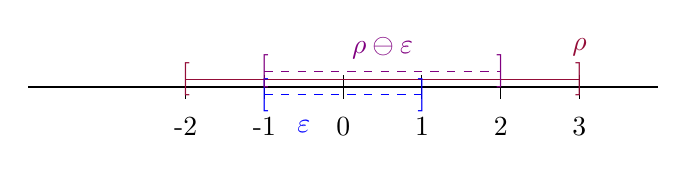
\begin{tikzpicture}
    \draw (-4,0) -- (4,0);

    \draw (0,-.15) -- (0,.15);
    \draw (-1,-.15) -- (-1,.15);
    \draw (-2,-.15) -- (-2,.15);
    \draw (1,-.15) -- (1,.15);
    \draw (2,-.15) -- (2,.15);
    \draw (3,-.15) -- (3,.15);
    \node at (0,-.5) {0};
    \node at (-1,-.5) {-1};
    \node at (1,-.5) {1};
    \node at (2,-.5) {2};
    \node at (3,-.5) {3};
    \node at (-2,-.5) {-2};

    \draw [cs] (-2,0.1) -- (3,0.1);
    \node [cs] at (3,.5) {$\rho$};
    \node [cs] at (-2,0.1) {\large [};
    \node [cs] at (3,0.1) {\large ]};

    \draw [blue,, dashed] (-1,-0.1) -- (1,-0.1);
    \node [blue] at (-.5,-.5) {$\varepsilon$};
    \node [blue] at (-1,-0.1) {\large [};
    \node [blue] at (1,-0.1) {\large ]};

    \draw [violet,, dashed] (-1,0.2) -- (2,0.2);
    \node [violet] at (.5,.5) {$\rho \ominus \varepsilon$};
    \node [violet] at (-1,0.2) {\large [};
    \node [violet] at (2,0.2) {\large ]};
  \end{tikzpicture}
  \caption{Opération de « rognage » $\ominus$ dans le cas des réels}
  \label{fig:rognage}
\end{figure}

\section{Application de portes}
\label{sec:Portes}

Il n'existe pas par défaut de formalisation des portes quantiques dans le cas de diagrammes de décision quantiques additifs abstraits, puisque cette structure de données est nouvelle. On a donc défini une application de portes $M \in \mathcal M_{2^n, 2^n}(\mathbb C)$ à un diagramme $D \in \mathcal D_n$ préservant ce qu'on attend comme effet sur l'évaluation des diagrammes, c'est-à-dire
$$\mathcal E(M(D)) = M \cdot \mathcal E(D)$$

\noindent où $\cdot$ est le produit matriciel basé sur le produit dans $\mathcal A_0$.
On note que, sans perte de généralité, on peut supposer que les coefficients de $M$ sont eux-mêmes des intervalles complexes. Réalisons un exemple d'application de porte sur un diagramme $D \in \mathcal D_n$.

\begin{figure}[ht]
  \centering
% https://tikzcd.yichuanshen.de/#N4Igdg9gJgpgziAXAbVABwnAlgFyxMJZAJgBoAGAXVJADcBDAGwFcYkQAREAX1PU1z5CKcqQCM1Ok1bsAMgH0xPPiAzY8BImPGSGLNohAK0y-uqFEAzDpp6ZhgEqLTqgRuHIALDan72TgFseSRgoAHN4IlAAMwAnCCDEURAcCCRtX3sQRmcaRnoAIxhGAAU3C0NYrDCACxwQPKwwAxAoejga0Jc4hKRk1KQyTJackzzC4rLzTUNGGGj6xub2No6u3hj4xP60xGth9ljc7InS8pmQKtr6jZAe7ZoBxG8Dyvkg8aKz6eFs+ZuVPd0o9dkM7AYwMxGIxPpNzr85gsGiBOvQoOxIMsli0oBAcDh1oCtkh9k8XuCkJDobDvoILojFiiYGiMQQ2NiVniCejuJRuEA
\begin{tikzcd}
  &     & D \arrow[lld, "l_1"', dashed] \arrow[ld, "l_p", dashed] \arrow[rd, "r_1"'] \arrow[rrd, "r_m"] &                                &     \\
L_1 \arrow[r, no head, dotted] & L_p &                                                                                               & R_1 \arrow[r, no head, dotted] & R_m
\end{tikzcd}
\caption{Diagramme $D$}
\label{fig:D_avant_porte}
\end{figure}

En pratique, pour appliquer une porte $M$ à un diagramme $D$
\begin{enumerate}
  \item On sépare $M$ en 4 sous-matrices
  $$M = \begin{pmatrix}
    M_{00} & M_{01} \\
    M_{10} & M_{11}
  \end{pmatrix}$$
  \item On crée pour chaque branche gauche de $D$ une branche droite  de même amplitude et pour chaque branche droite de $D$ une branche gauche de même amplitude.
  \item On applique $M_{00}$ à chaque branche gauche (hors celles créées à l'étape 2)
  \item On applique $M_{01}$ à chaque branche gauche (uniquement celles créées à l'étape 2)
  \item On applique $M_{10}$ à chaque branche droite (uniquement celles créées à l'étape 2)
  \item On applique $M_{11}$ à chaque branche droite (hors celles créées à l'étape 2)
\end{enumerate}

\begin{figure}[H]
  \centering
  % https://tikzcd.yichuanshen.de/#N4Igdg9gJgpgziAXAbVABwnAlgFyxMJZAFgBoAGAXVJADcBDAGwFcYkQBZACgBEBKEAF9S6TLnyEU5UgEZqdJq3YcA+sHLlBXADIqZA4aOx4CRGbPkMWbRJzUatutAZEgMxiUQBMFmlaW2quoyWgBKei5G4qYoAMy+CtbK9iFc4QC2kW5iJpLIAKwJ-jZ2wDKaOhFCru7ReQBsRYolQeWOKs7VUblEAOxNSYFqMqnh+l3ZHjHIABwDAaUjYSqZQvIwUADm8ESgAGYAThDpSNIgOBBI8YkBYMyMjDSM9ABGMIwACjmetowwezgQE8sGASlB6HAABYbCaHY6nGgXJBkG42O4PJ6vd5fKaSEB-AFA-EgsEQ6FQWFHE6IM5IxCFVFIdGPfFYz7fGL4-6AwwgOHU2mXRCNRmIZmYt7s3HsAk81z8hHnIU+UXi1mSnF1GXcomMEnscFQmG8hU0xFC8yq+4s54ajl42W6-W2Q3kynws1KpD9K0Y9XY+3awkmqmKulzX02tmanq-HUhj2Wukq4pM60SgPSuOEmjQ+gU2yQUFO4suiA4HDG+WhxDXOko1Ni9P+qVa7OA3MwfPsItsYGlkBQcuVikJ6kMukixtq22ZttcnMgPMF8AEPvEgdDitV-Y1n3hvzNNN+2et2MLjtLrsr3slsHD42UQRAA
\begin{tikzcd}[column sep=0.4cm, row sep=1.2cm]
  &             &                                        &             & M(D) \arrow[lld, dashed] \arrow[ld, dashed] \arrow[rd] \arrow[rrd] \arrow[llld, dashed] \arrow[lllld, dashed] \arrow[rrrd] \arrow[rrrrd] &                                        &             &                                        &             \\
M_{00}(L_1) \arrow[r, no head, dotted] & M_{00}(L_p) & M_{01}(R_1) \arrow[r, no head, dotted] & M_{01}(R_m) &                                                                                                                                          & M_{10}(L_1) \arrow[r, no head, dotted] & M_{10}(L_p) & M_{11}(R_1) \arrow[r, no head, dotted] & M_{11}(R_m)
\end{tikzcd}
  \caption {Diagramme $M(D)$}
  \label{fig:D_apres_porte}
\end{figure}

L'évaluation de $M(D)$ avec cet algorithme est correcte, puisque comme décrit sur la \autoref{fig:D_apres_porte}, on a
$$\mathcal E(M(D)) = \begin{pmatrix}
  \sum l_i M_{00} \mathcal E (L_i) + \sum r_j M_{01} \mathcal E (R_j) \\
  \sum l_i M_{10} \mathcal E (L_i) + \sum r_j M_{11} \mathcal E (R_j)
\end{pmatrix} = M \cdot \mathcal E (D)$$
\noindent ce qui correspond bien à l'effet attendu de l'application de la porte $M$ sur le diagramme $D$. Le cas de base (une matrice de taille 1, c'est-à-dire un scalaire) est traité simplement en multipliant les poids des branches par ce scalaire.

On a traité ici le cas d'une porte s'appliquant à tous les qubits. Plus généralement, considérant une porte s'appliquant seulement à $k$ qubits contigus (disons les qubits $Q ={q, ..., q+k-1}$). Pour un état $v$ à $n$ qubits, appliquer la porte $P \in \mathcal M_{2^k, 2^k}(\mathbb C)$ à aux qubits $Q$ de $v$ revient à appliquer à $v$ tout entier la porte

$$M = \left(\bigotimes^{q-1} I\right) \otimes P \otimes \left(\bigotimes^{n-k-q-1} I\right)$$

On remarque donc que l'application d'une porte à un nombre restreint de qubits peut être vue comme l'application d'une porte à tous les qubits, mais avec des matrices identités à la place des matrices de la porte.
De plus, utiliser des portes $S$ afin d'échanger la place de qubits permet de traiter avec l'algorithme présenté précédemment tous les cas d'application de portes logiques à un sous-ensemble quelconque des qubits du circuit.


\newpage

\chapter{Implementation}
\label{ch:Implementation}

The implementation was written in \textbf{C++}. This choice was motivated by several factors: performance, the maturity of the language and its use in several historical projects in the field \cite{Bichsel_2023} \cite{QTranslator}, and its proximity to the well-known C language.

\section{Structure du code}

The code is the subject of extensive documentation, available online. \cite{Leroy_doc}
The implementation makes extensive use of \textbf{object-oriented programming}, defining classes for the objects handled.
Some of the main classes are as follows, from lowest to highest level:
\begin{itemize}
  \item Real intervals (any, of positive reals or modulo $2\pi$), and complex intervals (Cartesian or polar)
  \item \textbf{Diagrams} (by default, additive and abstract)
  \item Branches, which contain a link (\textbf{pointer}) to a destination digram and a complex interval (Cartesian or polar)
\end{itemize}

Classes and functions are organized in \textbf{namespaces} to avoid name conflicts, and defined in separate files. \textbf{reduction} functions are then used to reduce diagrams, using selection functions.

The definition of functions and methods and their implementation are separated into header files and source code files, respectively. To take advantage of \textbf{separate compilation}, header files are included in source code files, and source code files are compiled into static libraries.

During this semester, an effort was made to improve \textbf{interchangeability} between Cartesian and polar intervals, and to make the code more generic, for example by defining adapted and optimized types for gate matrices or states (containing complexes or intervals).

\section{Tests}

To guarantee code quality, \textbf{unit tests} have been written for most functions and methods. These tests are written using the open-source \textit{Google Test} library, and are organized into \textbf{test suites} for each class. \cite{GoogleTest} The 46 tests, which run in less than half a second and include several thousand assertions, are used to validate code and detect bugs or regressions.

\section{QASM interpreter}

An \textbf{interpreter} for the Open QASM language was developed during this semester. It can be used to read a QASM file defining qubits and applying quantum gates to them, generate a diagram and make the modifications corresponding to the gates you wish to apply to it, and display the evaluation.

This interpreter can also operate in interactive mode, i.e. reading instructions from standard input. It does not support all QASM instructions, only basic logic gates ($X$, $H$, $CX$, $S$, phase gates). However, this interpreter's \textit{back-end} is capable of applying any gate using the method detailed in \autoref{sec:Portes}. This interpreter consists of a library that can be included with the header \texttt{qasm.h} including a \texttt{qasm} namespace and an \texttt{prompt} executable.

As QASM is already a quantum circuit description language, oppositely to a high-level programming language, it was not considered necessary to build a true compiler comprising a front-end, a middle-end performing optimizations and a back-end transforming the intermediate representation into an executable. The interpreter has been successfully tested on several examples of quantum circuits.

The example program \ref{lst:QASM} runs in 2.6 ms. \textbf{benchmarks} on a larger number of qubits, or on more complex circuits, have not been carried out. Furthermore, it is likely that a significant part of the execution time is due to reading the file or interpreting the QASM, and not to generating the diagram and modifying it.

\section{Tools}

The source code is versioned using \textit{Git}, and is available on the \textit{GitHub} platform. \cite{Git} \cite{GitHub} \cite{Leroy_2025} This project is the subject of a \textbf{continuous integration} using \textit{GitHub Actions}, automating test validation.

This semester saw the arrival of \textit{Clang} as a compiler instead of \textit{GCC}, and \textit{Ninja} instead of \textit{Make}. \cite{Clang} \cite{Ninja}
These changes have reduced compilation time and improved the readability of error messages, as well as facilitating the use of recent language features (dating back to C++23).
These tools are orchestrated by \textit{CMake}. \cite{CMake}

Compiling the project (excluding tests) takes about 8 seconds on a recent laptop. It takes a further 5 seconds to compile the tests. The project has around 5,000 lines of code, including around 1,000 lines of tests.

The project is also the subject of a \textbf{documentation}, written in the comments of the header files. Documentation web pages are automatically generated by \textit{Doxygen}. \cite{Doxygen} and automatically published on \textit{GitHub Pages} each time they are modified using \textit{GitHub Actions}. \cite{Leroy_doc}

\newpage


\chapter{Conclusion} % 1 page max
\label{ch:Conclusion}

\section{Travail réalisé}

Le modèle qui a été développé, avec algorithme de réduction, permet de limiter autant que souhaité la taille d'un état en mémoire, au prix d'une perte de précision. Le cadre mathématique de celui-ci a été défini, et des algorithmes de réduction ont étés prouvés sur cette structure de données.

L'implémentation, n'a pas encore fourni de résultats expérimentaux significatifs, mais permet déjà de simuler des diagrammes de décision quantiques de manière performante. Sa robustesse est assurée par des tests unitaires.

Au cours de ce semestre, des efforts sur l'implémentation ont été réalisés, entre autres afin de rendre interchangables les intervalles complexes cartésiens et polaires mais aussi plus généralement pour améliorer la qualité et réusabilité du code. La documentation du code a été améliorée, et le document principal détaillant les aspects théoriques du projet a été complété.

Un interpréteur QASM a été réalisé au cours de ce semestre, se reposant sur des travaux théoriques ayant permis une implémentation de l'application de portes à des diagrammes.

Le travail réalisé sur cette période est donc prometteur, et s'incrit dans la continuité du travail réalisé au semestre dernier : malgré des difficultés rencontrées, tant d'un point de vue technique en programmation que dans la définition du modèle, ayant parfois amené à revenir en arrière avant de trouver une bonne définition de l'erreur par exemple, les résultats théoriques obtenus sont prometteurs.

\section{Perspectives}

Plusieurs perspectives peuvent être envisagées pour prolonger les travaux réalisés. D'une part, puisque plusieurs choix dans la définition du modèle ont étés faits de manière arbitraire parmi plusieurs options possibles, il est pertinent de réaliser de nombreuses simulations dans des configurations différentes afin de déterminer les choix les plus pertinents.

On pourra notamment réaliser des tests de performance sur plusieurs fonctions d'erreur, ou observer l'effet d'échanges de qubits sur les performances en termes de manque de précision. De manière générale, il manque des \textbf{résultats expérimentaux} et en particulier des comparaisons à d'autres implémentations de la littérature sur des exemples usuels.

Nous pourrons aussi étendre le modèle avec d'autres concepts, comme les automates d'arbres pour la \textbf{vérification} ou les diagrammes de décisions et applications localement inversibles. \cite{Chen_2023} \cite{Vinkhuijzen_2023} Enfin, l'implémentation aurait à gagner d'être plus facile d'utilisation, par exemple avec une \textbf{interface graphique} pouvant agrémenter l'interpréteur QASM. Ces axes de travail pourront être explorés au cours de la suite du projet s'il est prolongé.

\newpage

% Hide page number for bibliography
\renewcommand{\thepage}{}


\printbibliography

\HRule \\[0.4cm]
\hfill{} \textsc{Malo \textsc{Leroy}} -- \textsc{CentraleSupélec} -- February 17${}^\text{th}$ 2025
\end{document}